\section{Permutations without repetition}

Combinatorics begins with arrangements. Imagine a row of empty places and a collection of distinct objects. We want to fill all places, using every object exactly once. In this situation, changing the order changes the result.

This is the most basic ordered counting scheme. It appears whenever the question is about arranging, ranking, scheduling, ordering, or placing all available distinct objects in a line.

\begin{definitionbox}
Let \(A\) be a finite set with \(n\) distinct elements. A permutation without repetition of the elements of \(A\) is an ordering of all elements of \(A\), in which every element appears exactly once.
\end{definitionbox}

For example, if
\[
A=\{a,b,c\},
\]
then the permutations without repetition are
\[
abc,\quad acb,\quad bac,\quad bca,\quad cab,\quad cba.
\]
There are six of them.

\begin{center}
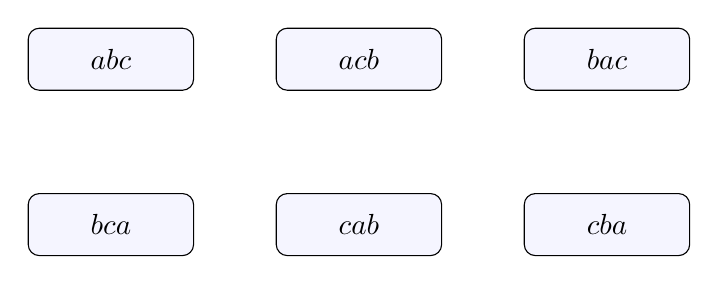
\begin{tikzpicture}[scale=1.05, transform shape]
\foreach \word/\x/\y in {abc/0/2, acb/3/2, bac/6/2, bca/0/0, cab/3/0, cba/6/0} {
    \node[draw, rounded corners, fill=blue!4, minimum width=2.0cm, minimum height=0.75cm] at (\x,\y) {$\word$};
}
\end{tikzpicture}
\end{center}

\begin{theorembox}
The number of permutations without repetition of \(n\) distinct elements is
\[
n! = n(n-1)(n-2)\cdots 2\cdot 1.
\]
\end{theorembox}

The formula follows directly from the multiplication principle. There are \(n\) choices for the first place. Once the first object has been used, there are only \(n-1\) choices for the second place. After two objects have been used, there are \(n-2\) choices for the third place. Continuing this reasoning gives
\[
n(n-1)(n-2)\cdots 2\cdot 1=n!.
\]

The decreasing number of choices is the signature of ``without repetition''. Each decision removes one object from later use.

\begin{examplebox}
Five different books are to be arranged on a shelf. Since all books are used, all books are distinct, and order matters, this is a permutation without repetition. The number of possible arrangements is
\[
5!=5\cdot4\cdot3\cdot2\cdot1=120.
\]
\end{examplebox}

\begin{examplebox}
Four students are to stand in a single line for a photograph. The students are distinct, every student stands in the line, and changing the order gives a different line. The number of possible lines is
\[
4!=24.
\]
\end{examplebox}

\begin{remarkbox}
Use permutations without repetition when all objects are distinct, all objects are used, and order matters. Typical words are: arrange, order, rank, line up, schedule all, place all.
\end{remarkbox}
